%Este trabalho está licenciado sob a Licença Atribuição-CompartilhaIgual 4.0 Internacional Creative Commons. Para visualizar uma cópia desta licença, visite http://creativecommons.org/licenses/by-sa/4.0/deed.pt_BR ou mande uma carta para Creative Commons, PO Box 1866, Mountain View, CA 94042, USA.

\chapter{Equação com uma incógnita}\label{cap_eq1d}
\thispagestyle{fancy}

Neste capítulo, discutiremos sobre métodos numéricos para resolver equações com uma incógnita real. Para tanto, notemos que toda equação pode ser reescrita na seguinte forma equivalente
\begin{equation}\label{eq:zero_fun}
  f(x) = 0,
\end{equation}
onde $f$ é uma função adequada. Isto é, o problema de se encontrar a incógnita de uma dada equação pode ser reescrito como um problema de encontrar os zeros (ou raízes) de uma função de uma variável real.

Os métodos numéricos que abordaremos ao longo deste capítulo são descritos para problemas da forma \eqref{eq:zero_fun}.

\section{Método da bisseção}\label{cap_eq1d_sec_bissec}

O método da bisseção explora o fato de que toda função contínua $f$ com $f(a)\cdot f(b) < 0$ (i.e., $f(a)$ e $f(b)$ tem sinais diferentes) tem pelo menos um zero no intervalo $(a, b)$\footnote{Esta é uma consequência imediata do \href{https://phkonzen.github.io/notas/AnaliseMatematicaI/cap_continuidade_sec_prop_f_cont.html}{teorema do valor intermediário}.}.

\begin{ex}\label{ex:bis_intro}
  Consideremos o problema de resolver
  \begin{equation}
    (2x^3-1,4x^2-0.98x+0.686)e^{-x^2} = (x^3-0,7x^2-0,49x+0,343)e^{-x^4}.
  \end{equation}
Este problema é equivalente a encontrar os zeros da seguinte função
\begin{align}
  f(x) &= (2x^3-1,4x^2-0.98x+0.686)e^{-x^2} \nonumber\\
       &- (x^3-0,7x^2-0,49x+0,343)e^{-x^4}.
\end{align}
Os zeros exatos\footnote{O problema foi construído para que tivesse estas soluções.} desta função são $x_1=-0,7$ e $x_2=x_3=0,7$ (veja a Figura \ref{fig:bis_intro}).

\begin{figure}[h!]
  \centering
  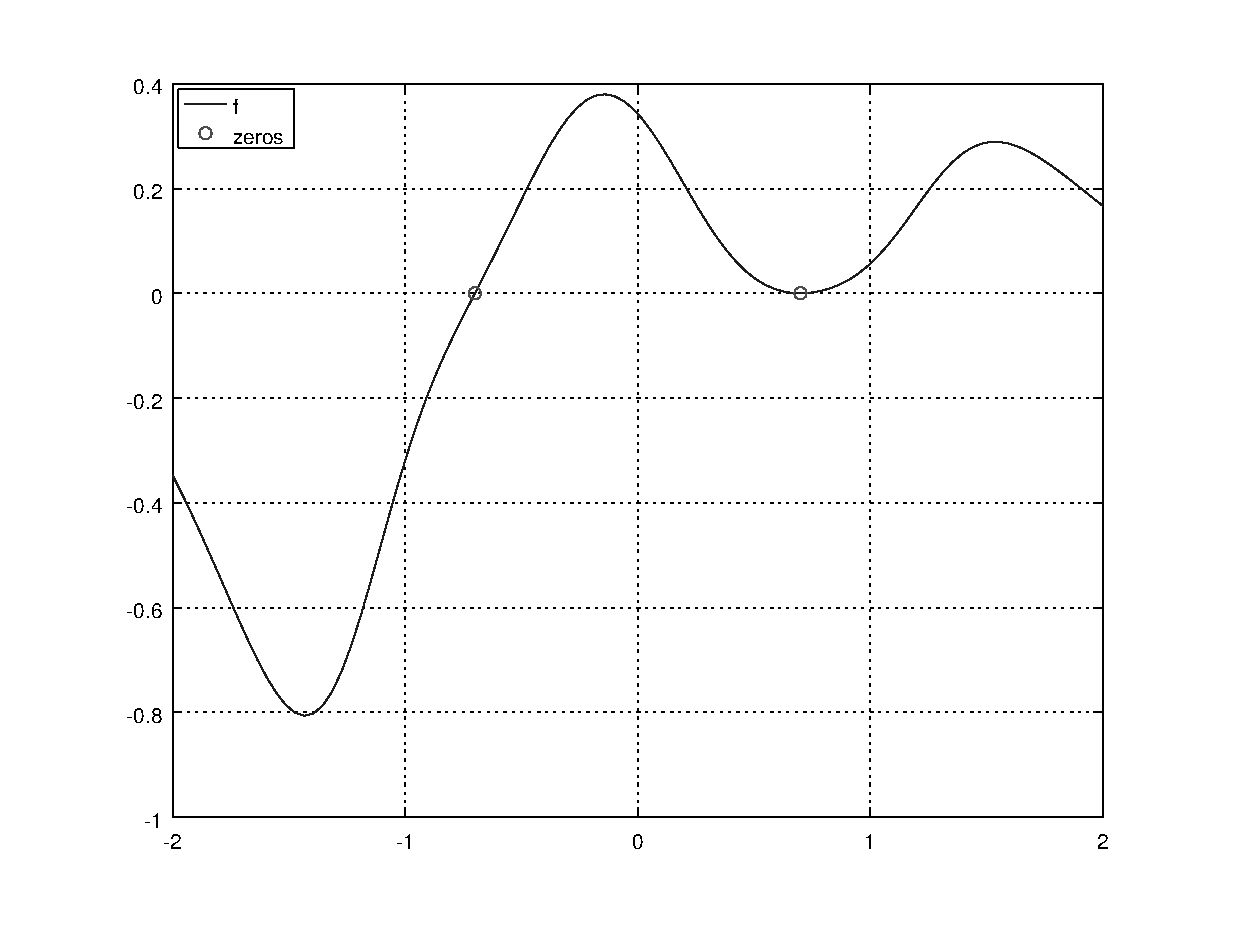
\includegraphics[width=0.8\textwidth]{./cap_eq1d/dados/ex_bis_intro/fig_bis_intro}
  \caption{Esboço da função $f$ do Exemplo~\ref{ex:bis_intro}.}
  \label{fig:bis_intro}
\end{figure}

Observamos que esta função é contínua e que, por exemplo, $f(-1)<0$ e $f(1)>0$, logo $f(-1)\cdot f(1) < 0$ e, de fato, $f$ tem pelo menos um zero\footnote{De fato, $f$ tem três zeros no intervalo $(-1, 1)$.} no intervalo $(-1, 1)$.

\ifisoctave
O esboço do gráfico da função $f$ pode ser feito no \verb+GNU Octave+ com o seguinte \href{https://github.com/phkonzen/notas/blob/master/src/MatematicaNumerica/cap_eq1d/dados/ex_bis_intro/ex_bis_intro.m}{código}:
\verbatiminput{./cap_eq1d/dados/ex_bis_intro/ex_bis_intro.m}
\fi
\end{ex}

Consideremos, então, uma função $f$ contínua tal que $f(a)\cdot f(b) < 0$. O método da bisseção é iterativo, sendo que a primeira aproximação para uma solução de $f(x)=0$ tomada como o ponto médio do intervalo $(a, b)$, i.e.
\begin{equation}
  x^{(1)} = \frac{a^{(1)}+b^{(1)}}{2},
\end{equation}
onde $a^{(1)} = a$ e $b^{(1)} = b$. Daí, se ocorrer $f(x^{(1)})=0$ o problema está resolvido. Caso contrário, $f$ tem pelo menos um zero num dos subintervalos $(a^{(1)}, x^{(1)})$ ou $(x^{(1)}, b^{(1)})$, pois $f(a^{(1)})\cdot f(x^{(1)}) < 0$ ou  $f(x^{(1)})\cdot f(b^{(1)}) < 0$, respectivamente e exclusivamente. No primeiro caso, escolhemos $(a^{(2)}, b^{(2)}) = (a^{(1)}, x^{(1)})$ ou, no segundo caso, tomamos $(a^{(2)}, b^{(2)}) = (x^{(1)}, b^{(1)})$. Então, a segunda aproximação para uma solução é computada como
\begin{equation}
  x^{(2)} = \frac{a^{(2)} + b^{(2)}}{2}.
\end{equation}
Daí, o procedimento se repete até obtermos uma aproximação com a precisão desejada.

\begin{ex}\label{ex:bis_exec}
  Consideremos o problema de encontrar um zero da função
  \begin{align}
  f(x) &= (2x^3-1,4x^2-0.98x+0.686)e^{-x^2} \nonumber\\
       &- (x^3-0,7x^2-0,49x+0,343)e^{-x^4}.
  \end{align}
Do esboço de seu gráfico (Figura \ref{fig:bis_intro}) vemos que $f(-1)\cdot f(1) \neq 0$. Então, aplicando o método da bisseção com intervalo inicial $(a^{(1)}, b^{(1)}) = (-1, 1)$ e aproximação inicial $x^{(1}) = (a^{(1)}+b^{(1)})/2$, obtemos as aproximações apresentadas na Tabela \ref{tab:bis_exec}.

Da Tabela \ref{tab:bis_exec}, observamos que as iteradas $x^{(k)}$ do método da bisseção parecem estar convergindo para o zero $x_1 = -0,7$ da função $f$. De fato, já na segunda iterada o método fica restrito a encontrar uma solução no intervalo $(a^{(2)}, b^{(2)}) = (-1, 0)$, o que excluí a possibilidade de o mesmo convergir para os outros zeros de $f$.

\begin{table}[h!]
  \centering
  \caption{Resultados referentes ao Exemplo~\ref{ex:bis_exec}.}
  \begin{tabular}{r|rr|r|c}
    k & $a^{(k)}$ & $b^{(k)}$ & $x^{(k)}$ & $f(a^{(k)})\cdot f(x^{(k)})$\\\hline
    1 & $-1,0000\E+0$ & $1,0000\E+0$ & $0,0000\E+0$ & -1 \\
    2 & $-1,0000\E+0$ & $0,0000\E+0$ & $-5,0000\E-1$ & -1 \\
    3 & $-1,0000\E+0$ & $-5,0000\E-1$ & $-7,5000\E-1$ & 1 \\
    4 & $-7,5000\E-1$ & $-5,0000\E-1$ & $-6,2500\E-1$ &  -1 \\
    5 & $-7,5000\E-1$ & $-6,2500\E-1$ & $-6,8750\E-1$ &  -1 \\
    6 & $-7,5000\E-1$ & $-6,8750\E-1$ & $-7,1875\E-1$ &  1 \\
    7 & $-7,1875\E-1$ & $-6,8750\E-1$ & $-7,0312\E-1$ & 1 \\
    8 & $-7,0312\E-1$ & $-6,8750\E-1$ & $-6,9531\E-1$ & -1 \\
    9 & $-7,0312\E-1$ & $-6,9531\E-1$ & $-6,9922\E-1$ & -1 \\
    10 & $-7,0312\E-1$ & $-6,9922\E-1$ & $-7,0117\E-1$ & 1 \\\hline
  \end{tabular}
  \label{tab:bis_exec}
\end{table}

\ifisoctave
A tabela \ref{tab:bis_exec} pode ser obtida no \verb+GNU Octave+ com o seguinte \href{https://github.com/phkonzen/notas/blob/master/src/MatematicaNumerica/cap_eq1d/dados/ex_bis_exec/ex_bis_exec.m}{código}:
\verbatiminput{./cap_eq1d/dados/ex_bis_exec/ex_bis_exec.m}
\fi
\end{ex}

\subsection{Análise de convergência}

Dada uma função estritamente monótona\footnote{Estritamente crescente ou estritamente decrescente.} e contínua $f:[a, b]\to\mathbb{R}$ com $f(a)\cdot f(b) < 0$, temos que o método da bisseção converge para o zero de $f$ no intervalo $(a, b)$. 

De fato, como consequência imediata do \href{https://phkonzen.github.io/notas/AnaliseMatematicaI/cap_continuidade_sec_prop_f_cont.html}{teorema do valor intermediário}, temos que $f$ tem pelo menos um zero no intervalo $(a, b)$. Agora, da hipótese de monotonicidade estrita, temos que $f$ tem um único zero neste intervalo, o qual denotaremos por $x^{*}$.

Da construção das iteradas do método, temos
\begin{align}
  |x^{(k)} - x^{*}| &\leq \frac{b^{(k)}-a^{(k)}}{2}\\
  &\leq \frac{b^{(k-1)}-a^{(k-1)}}{2^2}\\
  &\vdots \\
  &\leq \frac{b^{(1)}-a^{(1)}}{2^k},
\end{align}
donde, temos a seguinte estimativa do erro de truncamento
\begin{equation}\label{eq:bis_est_trunc}
  |x^{(k)} - x^{*}| \leq \frac{b^{(1)}-a^{(1)}}{2^k}.
\end{equation}
E, daí também, segue a convergência do método da bisseção, pois
\begin{equation}
  \lim_{k\to\infty} |x^{(k)}-x^{*}| = \lim_{k\to\infty} \frac{b^{(1)}-a^{(1)}}{2^k} = 0.
\end{equation}

\begin{obs}
  No caso de $f$ não ser estritamente monótona no intervalo $(a, b)$, ainda podemos garantir a convergência do método da bisseção. Isto segue do fato de que após algumas iteradas, digamos $k$ iteradas, a função $f$ terá apenas um zero no intervalo $(a^{(k)}, b^{(k)})$. A partir daí, as estimativas acima podem ser aplicadas.
\end{obs}

\begin{ex}\label{ex:bis_conv}
  No Exemplo \ref{ex:bis_exec} aplicamos o método da bisseção para a função
  \begin{align}
  f(x) &= (2x^3-1,4x^2-0.98x+0.686)e^{-x^2} \nonumber\\
       &- (x^3-0,7x^2-0,49x+0,343)e^{-x^4}.
  \end{align}
no intervalo $(-1, 1)$. Observando os resultados mostrados na Tabela \ref{tab:bis_exec}, vemos que
\begin{equation}
  |x^{(10)}-x^*| = 1,1719\E-3,
\end{equation}
com $x^* = x_1 = -0,7$. Observamos que este resultado está de acordo com a estimativa do erro de truncamento \eqref{eq:bis_est_trunc}, da qual temos
\begin{align}
  |x^{(10)} - x^*| &\leq \frac{b^{(1)}-a^{(1)}}{2^{10}}\\
  &= \frac{2}{2^{10}} = 1,9531\E-3.
\end{align}
\end{ex}

\begin{obs}(\normalfont{Taxa de convergência.})
  A estimativa de convergência \eqref{eq:bis_est_trunc} também pode ser usada para mostrarmos que, assintoticamente, o método da bisseção tem a seguinte taxa de convergência linear
  \begin{equation}
    \left|x^{(k+1)} - x^{(k)}\right| \lesssim \frac{1}{2}\left|x^{(k)} - x^{(k-1)}\right|^{\pmb{1}}.
  \end{equation}
\end{obs}

\subsection{Zeros múltiplos}

Sejam $f$ uma função suave e $x^*$ um zero de multiplicidade par de $f$. Observamos que o método da bisseção não é diretamente aplicável para aproximar $x^*$. Isto ocorre, pois, neste caso, $x^*$ será um ponto de mínimo ou de máximo local de $f$, não havendo pontos $a$ e $b$ próximos de $x^*$ tal que $f(a)\cdot f(b) < 0$.

Agora, sendo $x^*$ é um zero de multiplicidade $2m$ de $f$, temos que ela admite a seguinte decomposição
\begin{equation}
  f(x) = (x-x^*)^{2m}g(x),
\end{equation}
onde $g$ é uma função suave e $g(x^*)\neq 0$. Daí, a derivada de $f$
\begin{equation}
  f'(x) = 2m(x-x^*)^{2m-1}g(x) + (x-x^*)^{2m}g'(x),
\end{equation}
tem $x^*$ como um zero de multiplicidade $2m-1$ (ímpar) e, desta forma, podemos aplicar o método da bisseção em $f'$ para aproximar $x^*$.

\begin{ex}\label{ex:bis_multpar}
  A função
  \begin{align}
  f(x) &= (2x^3-1,4x^2-0.98x+0.686)e^{-x^2} \nonumber\\
       &- (x^3-0,7x^2-0,49x+0,343)e^{-x^4}.
  \end{align}
tem $x=0,7$ como um zero de multiplicidade par (veja Figura \ref{fig:bis_intro}). Para aplicarmos o método da bisseção para aproximarmos este zero, primeiramente, derivamos $f$
\begin{align}
  f'(x) &= \left(\left(6.0 x^{2} - 2.0 x \left(2.0 x^{3} - 1.4 x^{2} - 0.98 x + 0.686\right)\right.\right. \nonumber \\
        &\left.\left. - 2.8 x - 0.98\right) e^{x^{4}} + \left(x^{3} \left(4.0 x^{3} - 2.8 x^{2} - 1.96 x + 1.372\right)\right.\right.\nonumber\\
        &\left.\left.- 3.0 x^{2} + 1.4 x + 0.49\right) e^{x^{2}}\right) e^{- x^{2} \left(x^{2} + 1\right)}
\end{align}
O esboço do gráfico de $f'$ (Figura \ref{fig:bis_multpar}) mostra que $f'(0,5)\cdot f'(1) < 0$. Então, aplicando o método da bisseção a $f'$ no intervalo inicial $(a^{(1)}, b^{(1)}) = (0,5, ~1)$, obtemos os resultados apresentados na Tabela~\ref{tab:bis_multpar}. Nesta tabela são apresentados as iteradas até a convergência da solução com precisão de $10^{-3}$.

\begin{figure}[h!]
  \centering
  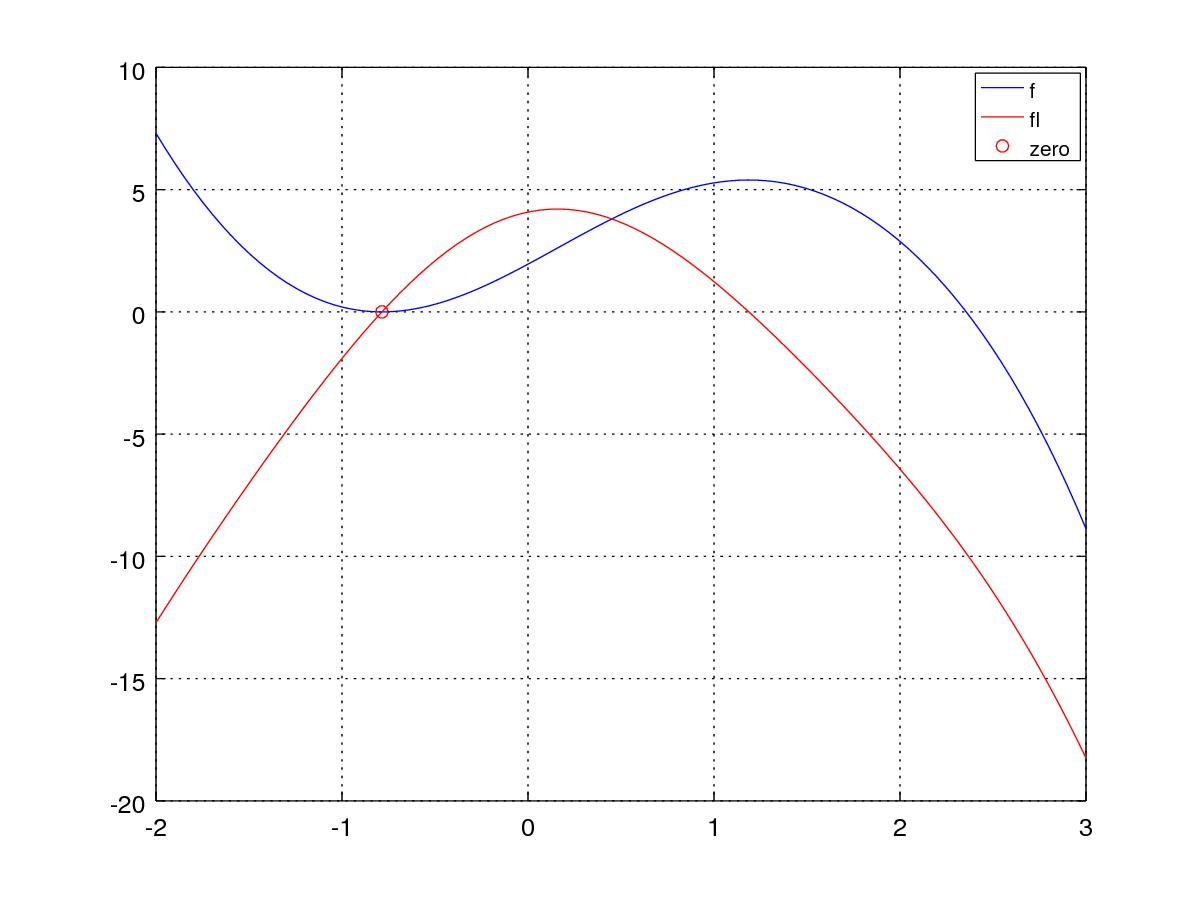
\includegraphics[width=0.8\textwidth]{./cap_eq1d/dados/ex_bis_multpar/fig_bis_multpar}
  \caption{Esboço do gráfico da derivada da $f$ dada no Exemplo \ref{ex:bis_multpar}.}
  \label{fig:bis_multpar}
\end{figure}
\end{ex}

\begin{table}[h!]
  \centering
  \caption{Resultados referentes ao Exemplo~\ref{ex:bis_exec}.}
  \begin{tabular}{r|rr|r|c}
    k & $a^{(k)}$ & $b^{(k)}$ & $x^{(k)}$ & $f'(a^{(k)})\cdot f'(x^{(k)})$\\\hline
    1 & $5,0000\E-1$ & $1,0000\E+0$ & $7,5000\E-1$ & -1 \\
    2 & $5,0000\E-1$ & $7,5000\E-1$ & $6,2500\E-1$ &  1 \\
    3 & $6,2500\E-1$ & $7,5000\E-1$ & $6,8750\E-1$ &  1 \\
    4 & $6,8750\E-1$ & $7,5000\E-1$ & $7,1875\E-1$ &  -1 \\
    5 & $6,8750\E-1$ & $7,1875\E-1$ & $7,0312\E-1$ &  -1 \\
    6 & $6,8750\E-1$ & $7,0312\E-1$ & $6,9531\E-1$ &  1 \\
    7 & $6,9531\E-1$ & $7,0312\E-1$ & $6,9922\E-1$ & 1 \\
    8 & $6,9922\E-1$ & $7,0312\E-1$ & $7,0117\E-1$ & -1\\
    9 & $6,9922\E-1$ & $7,0117\E-1$ & $7,0020\E-1$ &  -1\\\hline
  \end{tabular}
  \label{tab:bis_multpar}

\ifisoctave
A tabela \ref{tab:bis_multpar} pode ser obtida no \verb+GNU Octave+ com o seguinte \href{https://github.com/phkonzen/notas/blob/master/src/MatematicaNumerica/cap_eq1d/dados/ex_bis_multpar/ex_bis_multpar.m}{código}:
\verbatiminput{./cap_eq1d/dados/ex_bis_multpar/ex_bis_multpar.m}
\fi
\end{table}

\subsection*{Exercícios}

\begin{exer}\label{exer:bis_1}
  Use o método da bisseção para aproximar um zero de $f(x)=x^3\sen(x)-\cos(x)$, aplicando como intervalo inicial $(a^{(1)}, b^{(1)}) = (0,5, ~1)$ e aproximação inicial $x^{(1)}=(a^{(1)}+b^{(1)})/2$. Faça, então, $6$ iterações de forma a obter a aproximação $x^{(7)}$ e forneça-a com $7$ dígitos significativos por arredondamento.
\end{exer}
\begin{resp}
    \ifisoctave 
  \href{https://github.com/phkonzen/notas/blob/master/src/MatematicaNumerica/cap_aritm/dados/exer_bis_1/exer_bis_1.m}{Código.} 
  \fi
  $9,179688\times 10^{-1}$
\end{resp}

\begin{exer}\label{exer:bis_est_trunc}
  Considere que o método da bisseção para aproximar um zero de $f(x)=x^3\sen(x)-\cos(x)$, aplicando como intervalo inicial $(a^{(1)}, b^{(1)}) = (0,5, ~1)$ e aproximação inicial $x^{(1)}=(a^{(1)}+b^{(1)})/2$. Use a estimativa de convergência \eqref{eq:bis_est_trunc}
  \begin{equation}
    \left|x^{(k)} - x^{*}\right| \leq \frac{b^{(1)}-a^{(1)}}{2^k},
  \end{equation}
para estimar o número mínimo de iterações $k_{conv}$ necessárias para se obter a solução com exatidão de $10^{-4}$. Então, compute $x^{(k_{conv})}$ e forneça-o com $6$ dígitos significativos por arredondamento.
\end{exer}
\begin{resp}
    \ifisoctave 
  \href{https://github.com/phkonzen/notas/blob/master/src/MatematicaNumerica/cap_aritm/dados/exer_bis_este_trunc/exer_bis_est_trunc.m}{Código.} 
  \fi
  $9,15833\E-1$
\end{resp}

\begin{exer}\label{exer:bis_multpar}
  Use o método da bisseção para encontrar uma aproximação com precisão de $10^{-4}$ do zero de
  \begin{equation}
    f(x) = (-x^2+1,154x-0,332929)\cos(x) + x^2 - 1,154x + 0,332929
  \end{equation}
no intervalo $(0,55, ~0,65)$. Forneça a aproximação computada com $7$ dígitos significativos por arredondamento.
\end{exer}
\begin{resp}
    \ifisoctave 
  \href{https://github.com/phkonzen/notas/blob/master/src/MatematicaNumerica/cap_aritm/dados/exer_bis_multpar/exer_bis_multpar.m}{Código.} 
  \fi
  $5,770508\times 10^{-1}$
\end{resp}

\section{Método da falsa posição}\label{cap_eq1d_sec_falsapos}

O método da falsa posição é uma variação do método da bisseção.

\begin{figure}[h!]
  \centering
  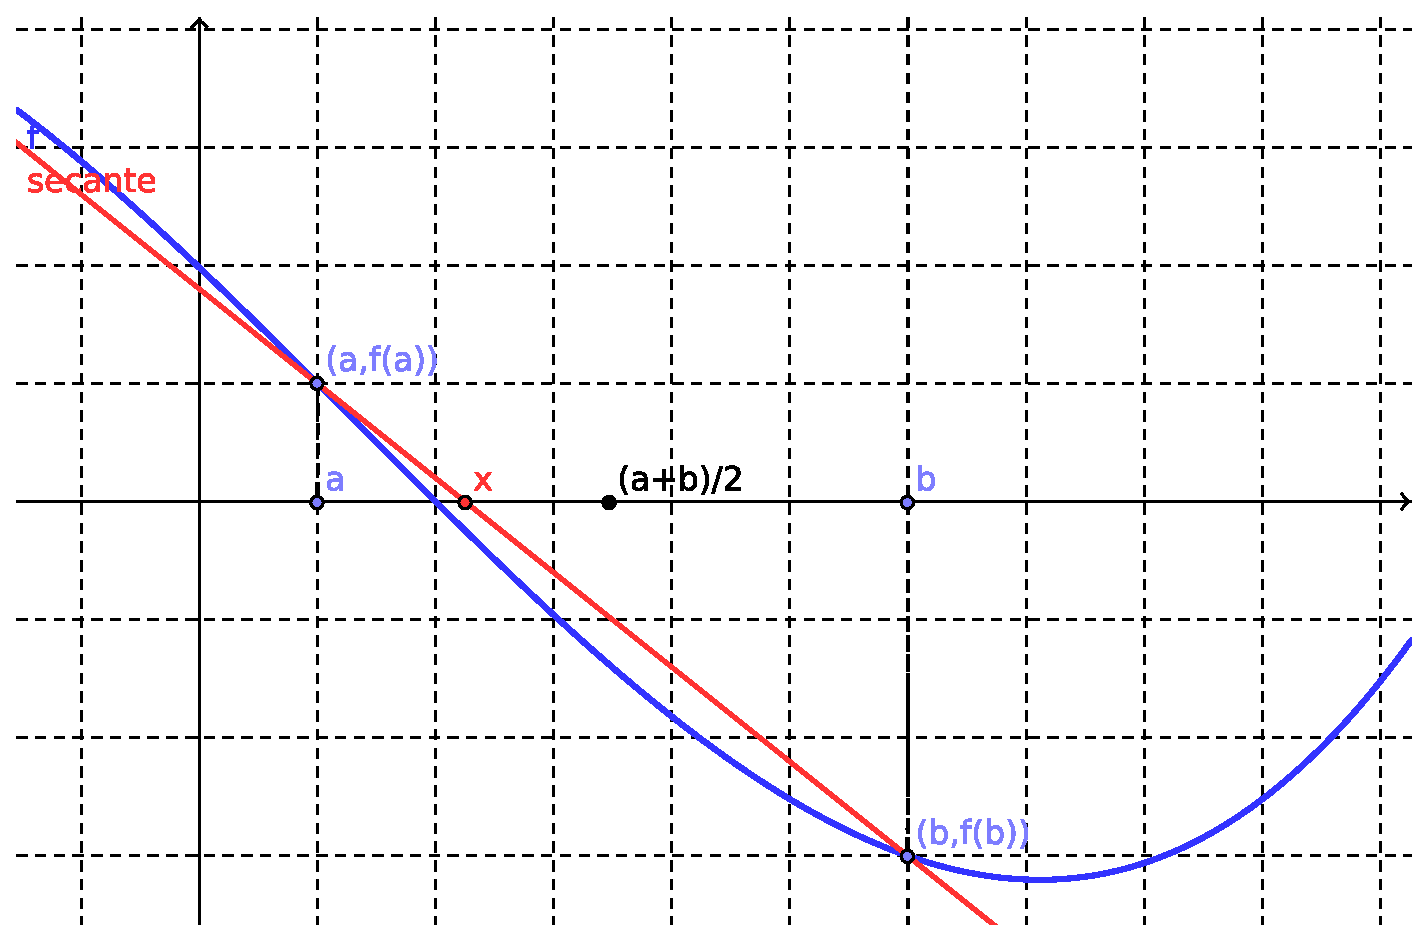
\includegraphics[width=0.7\textwidth]{./cap_eq1d/dados/fig_falsapos/fig_falsapos}
  \caption{Ilustração do método da falsa posição (veja no \href{https://github.com/phkonzen/notas/blob/master/src/MatematicaNumerica/cap_eq1d/dados/fig_falsapos/fig_falsapos.ggb}{Geogebra}.}
  \label{fig:falsapos}
\end{figure}

\emconstrucao